\chapter{Systemaufbau und Umsetzung}
\label{ch:systemaufbau}
\section{Technikstand Fahrrad \(Bellgardt, Menzel\)}
\label{sec:technikstandfahrrad}
Der Fahrradaufbau dient zur Erfassung von Kräften am Fahrradlenker, indem mechanische Größen in elektrische Signale umgewandelt werden.
Dazu werden Dehnungsmessstreifen (DMS) verwendet, die auf relevante Bauteile aufgeklebt werden, um dort auftretende Verformungen zu erfassen.
In einer Messbox befindet sich die Messtechnik. Diese zeichnet über die Zeit dann die Belastung auf. Insgesamt befinden sich an dem Lenker 8 DMS.
Auf jeder Lenkerseite gibt es jeweils zwei DMS welche als Halbbrücke geschalten sind und die Kräfte in horizontaler oder vertikaler Richtung messen. 
Abbildungen \ref{fig:fab3} und \ref{fig:fab4} zeigen den alten Aufbau des Fahrrads.
Um den alten Versuchsaufbau bei Bedarf wiederherstellen zu können musste dieser genau dokumentiert werden.
Dies geschah durch das Beschriften der in der Lenkerbox befindlichen Kabel, siehe \todo{Anhang}


An dem bisherigen Aufbau wurden folgende Optimierungsmöglichkeiten erkannt:
\begin{itemize}
    \item Bisheriger Aufbau am Fahrrad kabelgebunden (USB-Kabel zu PC)
    \item Keine Zugentlastung an der Lenkerbox
    \item Nicht spritzwassergeschützt
    \item Zwischenplatine benötigt
    \item Kontaktierung durch Verschraubung
\end{itemize}

\begin{figure}[htbp]
    \begin{center}
        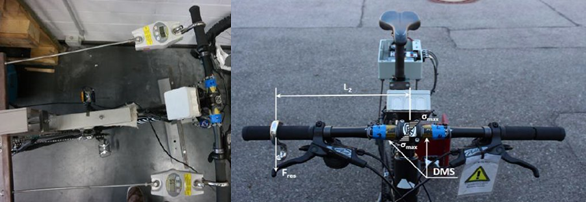
\includegraphics[width=1.0\textwidth, keepaspectratio]{fab3.png}
        \caption[Alter Aufbau des Fahrrads, Lenker (Abbildungsverzeichnis)]{Alter Aufbau des Fahrrads, Lenker
        \footcite{Rechter Teil des Bildes: Praktikum Schwingbruchgefaehrdete Bauteile sicher dimensionieren und betreiben
        }
        }
        \label{fig:fab3}
    \end{center}
\end{figure}


\begin{figure}[htbp]
    \begin{center}
        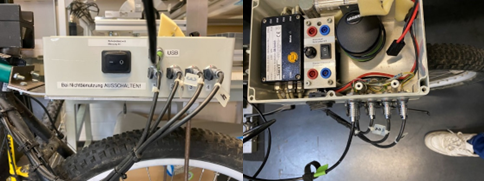
\includegraphics[width=1.0\textwidth, keepaspectratio]{fab4.png}
        \caption[Alter Aufbau des Fahrrads, Messbox (Abbildungsverzeichnis)]{Alter Aufbau des Fahrrads, Messbox}
        %\footcite{Rechter Teil des Bildes: Praktikum Schwingbruchgefaehrdete Bauteile sicher dimensionieren und betreiben
        %}
        
        \label{fig:fab4}
    \end{center}
\end{figure}


\newpage
\section{Wahl der Komponenten \(Nerb, Ulit\)}
Für die Umsetzung des Messsystems wurden verschiedene Komponenten sorgfältig ausgewählt, um eine zuverlässige und robuste Datenerfassung zu gewährleisten. Dabei wurden insbesondere folgende Kriterien berücksichtigt: Präzision der Messwerte, Widerstandsfähigkeit gegenüber äußeren Einflüssen sowie eine einfache Integration der Bauteile in das Gesamtsystem.
Die wichtigsten gewählten Komponenten umfassen:
\begin{itemize}
    \item \textbf{V-Link 200}: Drahtloses Datenerfassungsmodul zur Übertragung der DMS-Signale.
    \item \textbf{Dehnungsmessstreifen (DMS)}: Zur Erfassung der mechanischen Verformungen, angepasst an die jeweiligen Messaufgaben (Biegung oder Torsion).
    \item \textbf{Metallschichtwiderstände (120 Ohm)}: Hochpräzise Widerstände zur Stabilisierung der Brückenschaltung.
    \item \textbf{Leiterplattenklemmen}: Erleichtern den Austausch und die Anpassung der Verdrahtung.
    \item \textbf{Spritzwassergeschütztes Gehäuse}: Dient zum Schutz der Elektronik gegen Umwelteinflüsse.
    \item \textbf{Acrylplatte zur Befestigung des V-Link 200}: Gewährleistet eine stabile Montage innerhalb des Gehäuses.
    \item \textbf{Steuerleitung (geschirmt, 4-adrig)}: Reduziert Störungen und sichert eine zuverlässige Signalübertragung.
    \item \textbf{Stecker und Buchsen (4-Pin und 3-Pin)}: Der 4-Pin-Stecker dient zur aktuellen Verdrahtung, während der 3-Pin-Stecker für zukünftige Anwendungen vorgesehen ist.
    \item \textbf{PG-7 Kabelverschraubung}: Dient zur Zugentlastung der Kabel und schützt die Verbindungen vor mechanischer Beanspruchung.
    \item \textbf{KFZ-Zigarettenanzünder-Steckdose mit Schutzkappe}: Ermöglicht einen Durchgriff ins Gehäuse, sodass der Einschaltknopf des V-Link gedrückt werden kann, ohne das Gehäuse zu öffnen.
\end{itemize}


\section{Einbau des V\-Link 200 in ein spritzwassergesch\"utztes Geh\"ause \(Nerb, Ulit\)}
Um den \textbf{V-Link 200} vor Umwelteinflüssen zu schützen und eine sichere Installation der Elektronik zu gewährleisten, wurde ein spritzwassergeschütztes Gehäuse gewählt. Dieses bietet ausreichend Platz für die Montage des V-Link sowie die notwendige Verdrahtung der angeschlossenen Komponenten.

Für die Befestigung des V-Link im Gehäuse wurde eine maßgefertigte \textbf{Acrylplatte} angefertigt. Diese wurde entsprechend der Innenmaße des Gehäuses angepasst und mit \textbf{M4-Feingewindeschrauben} verschraubt. Zusätzlich wurde ein Ausschnitt für den Einschaltknopf des V-Link vorgesehen, um eine einfache Bedienung zu ermöglichen.
\subsection{Montageschritte}

\begin{enumerate}
    \item Vermessung des Gehäuses und Anfertigung der Acrylplatte mit CAD-Software.
    \item Laserschneiden der Acrylplatte und Anbringung der notwendigen Bohrungen.
    \item Bohren der Gehäuseöffnungen für die Steckerbuchsen und den Durchgriff für den Einschaltknopf.
    \item Löten der Kabel an die Buchsen und Verbindung mit dem V-Link 200.
    \item Befestigung des V-Link 200 mit Feingewindeschrauben und Muttern.
    \item Montage der Acrylplatte im Gehäuse mit Flachkopfschrauben.
    \item Verdrahtung des V-Link 200 mit den Steuerleitungen.
    \item Sicherung der Kabel zur Vermeidung von mechanischen Belastungen.
\end{enumerate}


Nach dem Einbau wurden abschließend alle Verbindungen geprüft, um sicherzustellen, dass der \textbf{V-Link 200} korrekt funktioniert und die \textbf{DMS-Signale} zuverlässig erfasst werden.
Abbildungen \ref{fig:un10} und \ref{fig:un11} zeigen das fertige Gehäuse.
\begin{figure}[htbp]
    \centering
    \begin{minipage}{0.48\textwidth}
        \centering
        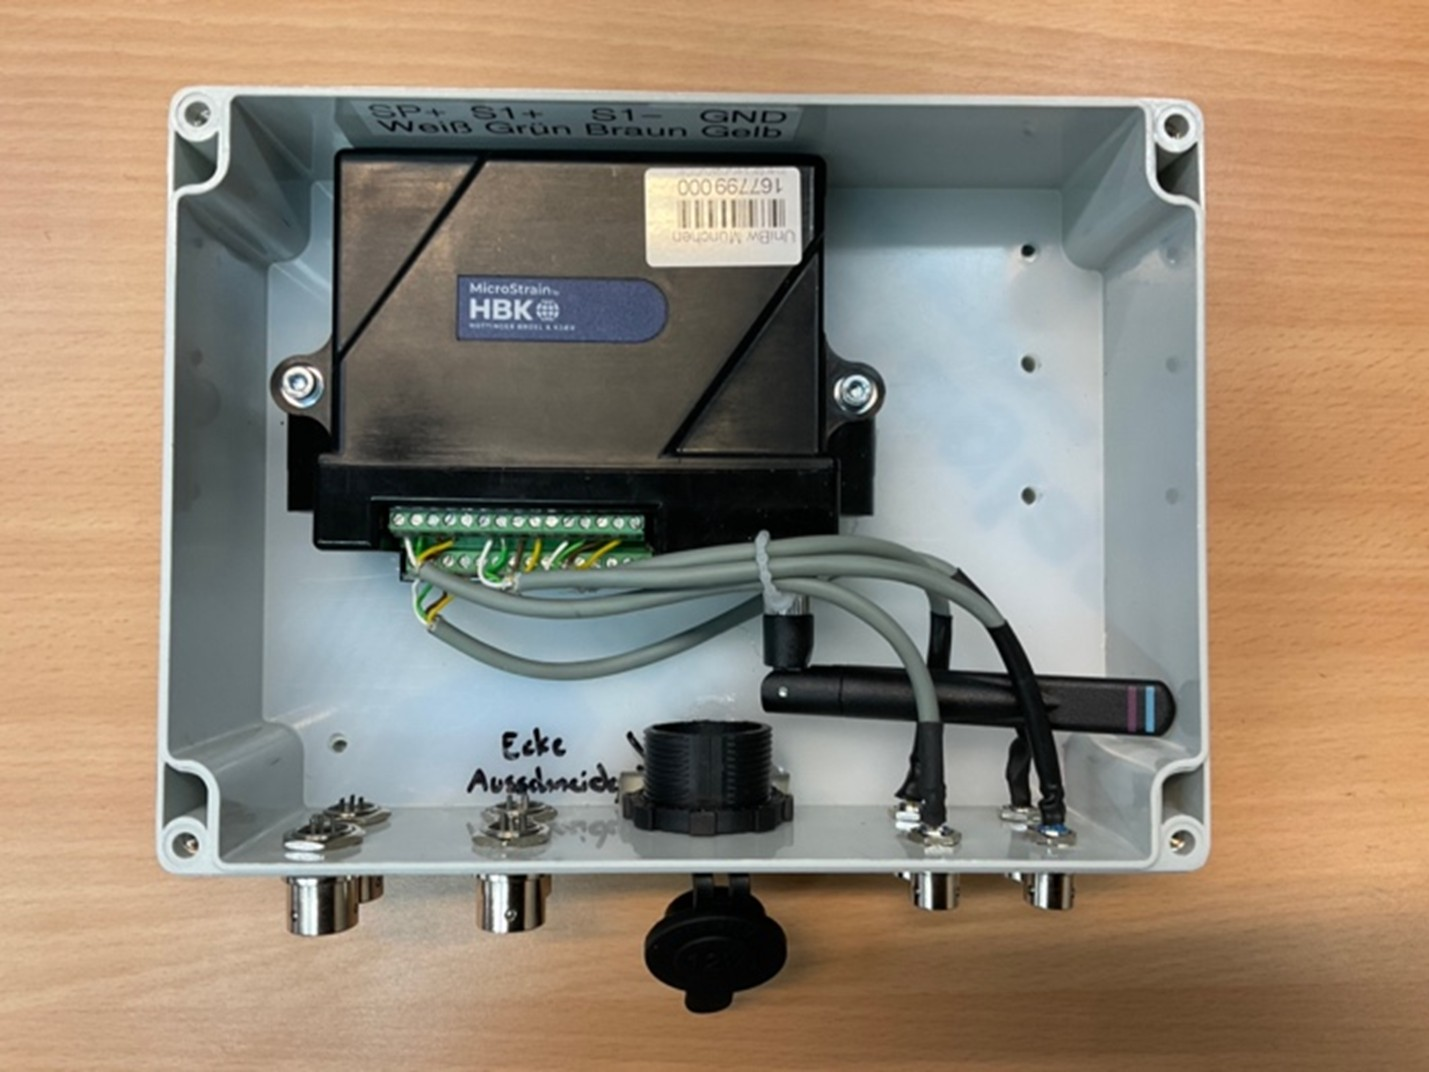
\includegraphics[width=\textwidth]{un10.jpg}
        \caption[Geh\"ause Ansicht Oben (Abbildungsverzeichnis)]{Geh\"ause Ansicht Oben}
        \label{fig:un10}
    \end{minipage}
    \hfill
    \begin{minipage}{0.48\textwidth}
        \centering
        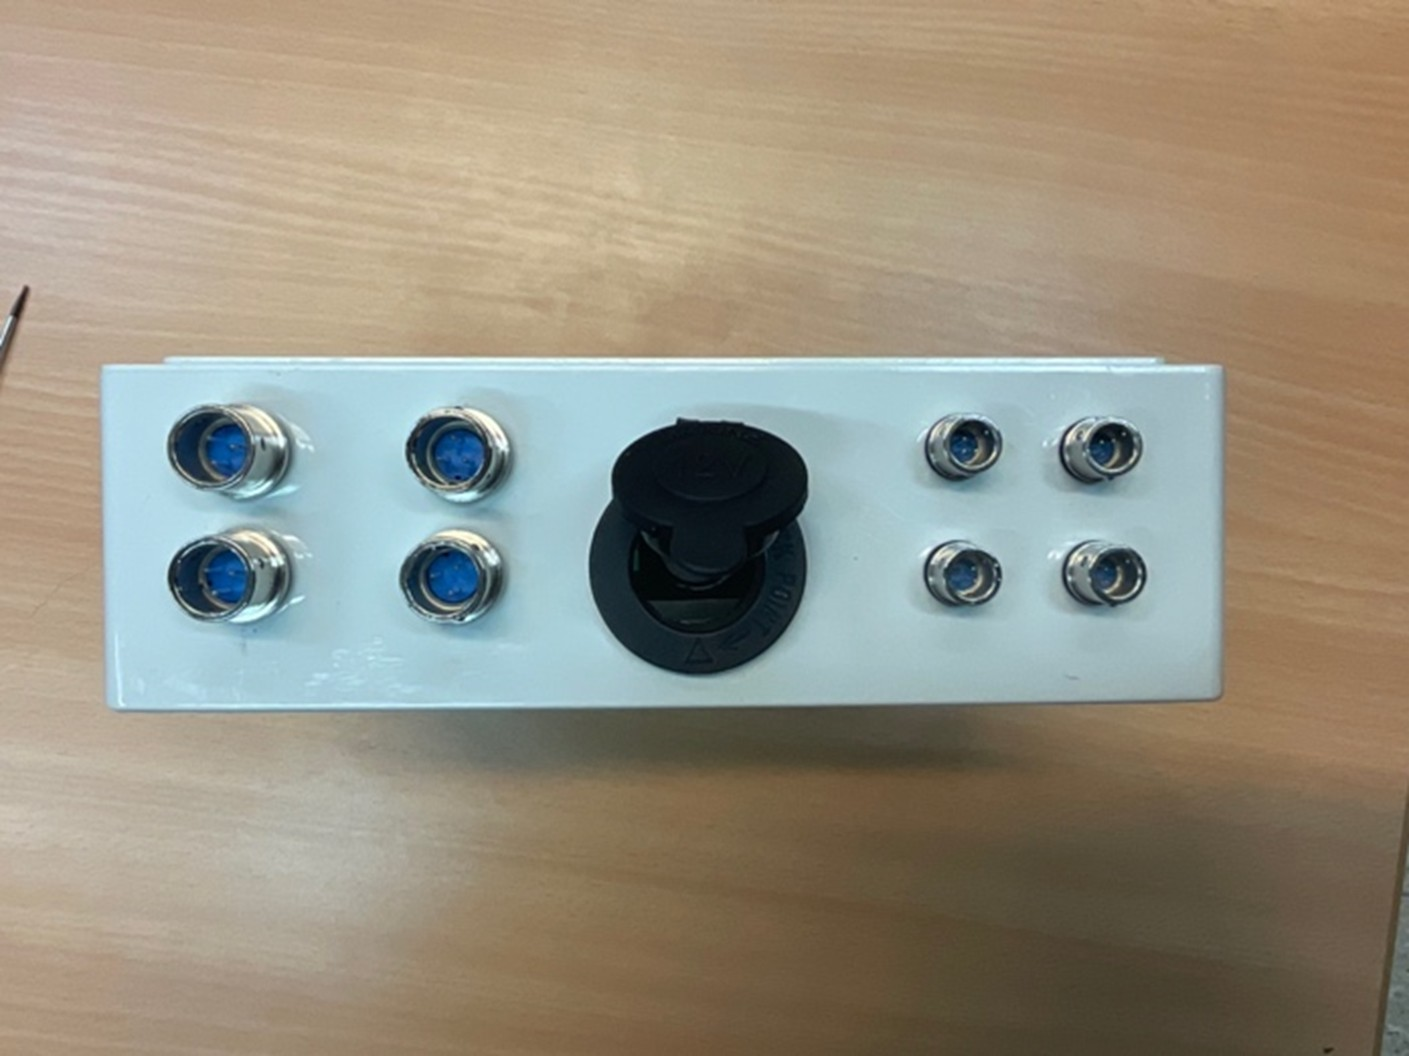
\includegraphics[width=\textwidth]{un11.jpg}
        \caption[Geh\"ause Ansicht Frontal (Abbildungsverzeichnis)]{Geh\"ause Ansicht Frontal}
        \label{fig:un11}
    \end{minipage}
    \caption{Unterschiedliche Ansichten des Gehäuses}
    \label{fig:gehaeuse_ansichten}
\end{figure}



\clearpage
\section{Entwurf der Schaltung und Platine}



\subsection{Umschalter f\"ur Halb- und Vollbr\"ucke (geplant, nicht umgesetzt) \(Nerb, Ulit\)}
Um eine hohe Flexibilität bei der Messwerterfassung zu gewährleisten, haben wir eine Schaltung geplant, die es ermöglichen sollte, zwischen einer Halb- und Vollbrückenschaltung umzuschalten, siehe Abbildung \ref{fig:un1}.
\begin{figure}[h]
    \begin{center}
        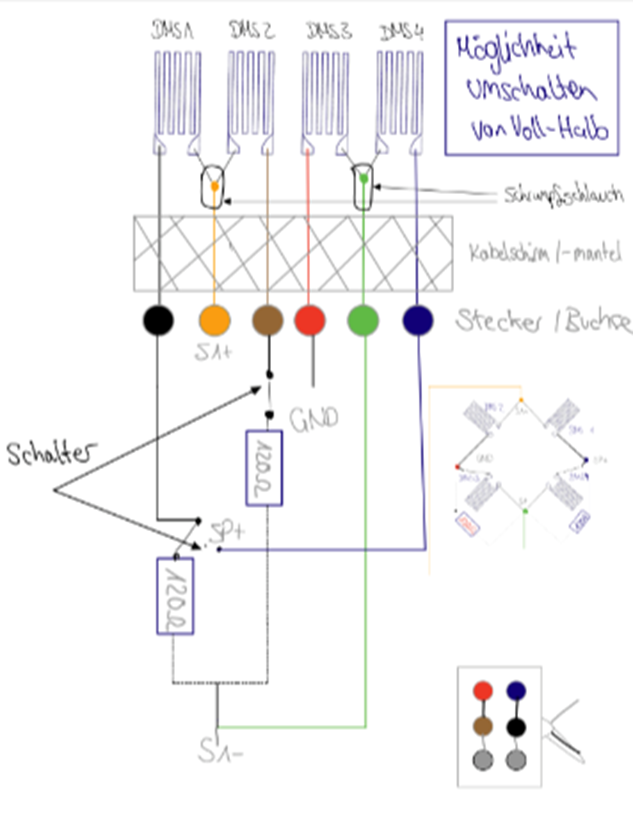
\includegraphics[width=0.5\textwidth, keepaspectratio]{un1.png}
        \caption[Umschalter f\"ur Halb- und Vollbr\"ucke (Abbildungsverzeichnis)]{Umschalter f\"ur Halb- und Vollbr\"ucke}
        %\footcite{VLInkManual}
        
        \label{fig:un1}
    \end{center}
\end{figure}

Diese Schaltung wurde jedoch nicht umgesetzt, da die Vorteile eines anderen Schaltung überwogen haben.
Die Idee basierte auf der Verwendung von zwei Kippschaltern des Typs MTS-202-A1, die die entsprechenden Widerstände in die Schaltung ein- oder ausschalten können.
Dadurch wäre es möglich gewesen, verschiedene Sensortypen anzuschließen, ohne dass eine neue Platine entwickelt oder neu verdrahtet werden müsste. 
Dies wird durch zwei Kippschalter des Typs MTS-202-A1 realisiert, die die entsprechenden Widerstände in die Schaltung ein- oder ausschalten können.
Diese Lösung bietet den Vorteil, dass verschiedene Sensortypen angeschlossen werden können, ohne dass eine neue Platine entwickelt oder neu verdrahtet werden muss.
Geplant war, die Platine direkt in der Messbox beim V-Link 200 zu integrieren, sodass kein zusätzliches Gehäuse für die Umschaltelektronik benötigt wird.
In der Planung war eine sechsadrige Steuerleitung mit einem Querschnitt von 0,14 mm² vorgesehen, wobei der Anschluss über einen sechspoligen Stecker mit Buchse erfolgen sollte,
um eine einfache und sichere Verbindung zu gewährleisten.
Dadurch wird vermieden, dass ein zusätzliches Gehäuse für die Umschaltelektronik benötigt wird.
Zur Verbindung zwischen den Komponenten haben wir eine sechsadrige Steuerleitung mit einem Querschnitt von 0,14 mm² eingeplant.
Der Anschluss erfolgt über einen sechspoligen Stecker mit Buchse, der eine einfache und sichere Verbindung gewährleistet.
Das begleitende Schaltbild zeigt den geplanten Aufbau der Verdrahtung der Dehnungsmessstreifen (DMS) sowie die Position der Widerstände und Schalter.
In der Theorie wären die DMS in einer Brückenschaltung angeordnet worden, wobei durch das Betätigen der Kippschalter verschiedene Konfigurationen hätten realisiert werden können.
Die Widerstände (120 Ohm) sollten je nach gewünschter Brückenschaltung aktiviert oder deaktiviert werden. (DMS) sowie die Position der Widerstände und Schalter.
Die DMS sind in einer Brückenschaltung angeordnet, wobei durch das Betätigen der Kippschalter verschiedene Konfigurationen realisiert werden können.
Die Widerstände (120 Ohm) werden dabei je nach gewünschter Brückenschaltung aktiviert oder deaktiviert.
\subsubsection{Vor- und Nachteile der Lösung}
\textbf{Vorteile}
\begin{itemize}
    \item Eine Platine für alle Schaltmöglichkeiten
    \item Möglichkeit zur Nutzung unterschiedlicher Sensortypen
    \item Schnelleres Umschalten ohne Neuverdrahtung oder Platinenwechsel
    \item Intuitive Bedienung
    \item Keine zusätzliche externe Gehäuseeinheit nötig
\end{itemize}

\textbf{Nachteile}
\begin{itemize}
    \item Fehlende Zugentlastung der Leitungen
    \item Funktioniert nur mit Sensoren, für die 120-Ohm-Widerstände passend sind
    \item Mechanische Schalter haben einen gewissen Übergangswiderstand, was zu minimalen Messabweichungen führen kann
    \item Zusätzlicher Platzbedarf und komplexe Verkabelung in der Messbox
    \item Potentielle Messfehler bei falscher Bedienung
\end{itemize}


Abbildung \ref{fig:un1} veranschaulicht die praktische Umsetzung dieser Schaltung.
Es zeigt die Dehnungsmessstreifen (DMS 1–4) sowie deren Verdrahtung zu einem geschirmten Kabelbündel.
Die Kippschalter befinden sich zwischen den Messleitungen und ermöglichen das Zu- oder Abschalten der Widerstände, wodurch sich die Brückenschaltung entsprechend anpassen lässt.
In der schematischen Darstellung im unteren Bereich ist zudem die Funktionsweise der Umschaltung verdeutlicht.




\subsection{Br\"uckenschaltung f\"ur zwei DMS \(Nerb, Ulit\)}
Um die Genauigkeit der Messungen zu gewährleisten, haben wir uns für den Einsatz von zwei Dehnungsmessstreifen (DMS) in einer Brückenschaltung entschieden.
Diese Konfiguration erlaubt eine präzisere Erfassung von Kräften und Dehnungen, da sich die Sensoren gegenseitig kompensieren können.
Zusätzlich zu den DMS haben wir zwei 120-Ohm-Metallschichtwiderstände in die Schaltung integriert.
Die Wahl von Metallschichtwiderständen erfolgte aufgrund ihrer hohen Langzeitstabilität und geringen Temperaturabhängigkeit, was für die Genauigkeit der Messungen entscheidend ist.
Die Schaltung wurde so entworfen, dass sie in einem separaten Platinengehäuse untergebracht ist, das zwischen der Messbox und den DMS angeordnet wurde.
Diese Trennung reduziert die Verkabelung in der Messbox und ermöglicht eine einfachere Wartung.
Ein weiterer Vorteil dieser Lösung ist die Reduzierung der benötigten Verkabelung.
Durch den Einsatz einer vieradrigen, geschirmten Steuerleitung konnten wir nicht nur das Gewicht der Messbox verringern, sondern auch die Störanfälligkeit minimieren.
Die Abschirmung schützt die Signalleitungen vor externen elektromagnetischen Einflüssen und sorgt so für zuverlässigere Messwerte.
Im Platinengehäuse erfolgt die Verschaltung der Widerstände, wodurch die Schaltung insgesamt übersichtlicher wird. Dies erleichtert die Fehleranalyse und Wartung.
Außerdem ermöglicht diese Lösung eine kostengünstige Herstellung der Platinen, da wir interne Ressourcen für den hochwertigen Platinenbau nutzen konnten. 

\subsubsection{Vor- und Nachteile der Lösung}
\textbf{Vorteile}
\begin{itemize}
    \item Kompakte Bauweise mit integrierter Zugentlastung
    \item Weniger Verkabelung durch den Einsatz einer vieradrigen, geschirmten Steuerleitung
    \item Höhere Messgenauigkeit durch den Einsatz einer Vollbrückenschaltung
    \item Reduzierung elektromagnetischer Störungen durch die geschirmte Leitung
    \item Einfachere Wartung und geringere Fehleranfälligkeit
    \item Kostengünstige Platinenherstellung durch interne Fertigung
\end{itemize}

\textbf{Nachteile}
\begin{itemize}
    \item Keine flexible Umschaltung auf andere Brückenarten möglich
    \item Höherer Platzbedarf innerhalb des Platinengehäuses
    \item Abhängigkeit von 120-Ohm-Widerständen für die Kalibrierung
\end{itemize}
Abbildung \ref{fig:un2} zeigt die vollständige Verdrahtung der beiden DMS sowie die Integration der Widerstände.
\begin{figure}[h]
    \begin{center}
        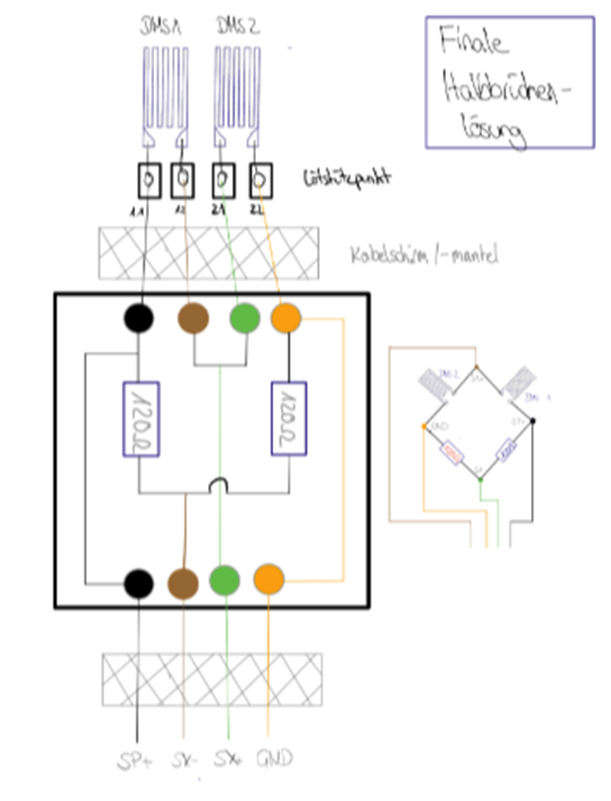
\includegraphics[width=0.5\textwidth, keepaspectratio]{un2.png}
        \caption[Finale Halbbr\"uckenl\"osung (Abbildungsverzeichnis)]{Finale Halbbr\"uckenl\"osung}
        %\footcite{VLInkManual}
        
        \label{fig:un2}
    \end{center}
\end{figure}
Die Signale werden innerhalb des Platinengehäuses verarbeitet, bevor sie an den V-Link 200 in der Messbox zur drahtlosen Übertragung weitergeleitet werden. Die schematische Darstellung in der unteren rechten Ecke veranschaulicht die genaue Schaltungskonfiguration.
\textbf{Hinweis:} Die schwarze Leitung in der Darstellung entspricht in unserer tatsächlichen Umsetzung einer weißen Leitung. Diese Anpassung wurde aus Gründen der besseren Übersichtlichkeit in der Schaltungsgrafik gewählt.




\newpage{}
\subsection{Lenkerbox Fahrrad \(Menzel\)}
Die alte Lenkerbox ist nicht spritzwassergeschützt, und die verwendeten Leitungen sind nicht geschirmt.
Zudem gibt es keine Zugentlastung der Leitungen zur Messtechnik.
Diese Punkte sollten bei der Auswahl und Umsetzung einer neuen Lenkerbox berücksichtigt werden.\
Um ausreichend Platz zum verlöten der Platine und DMS zu haben wurde zunächst eine Box mit IPP6 Schutz und den Aussenmassen mit  122 x 120 x 55mm gewählt, siehe Abbildung \ref{fig:box1}.

\begin{figure}[h]
    \begin{center}
        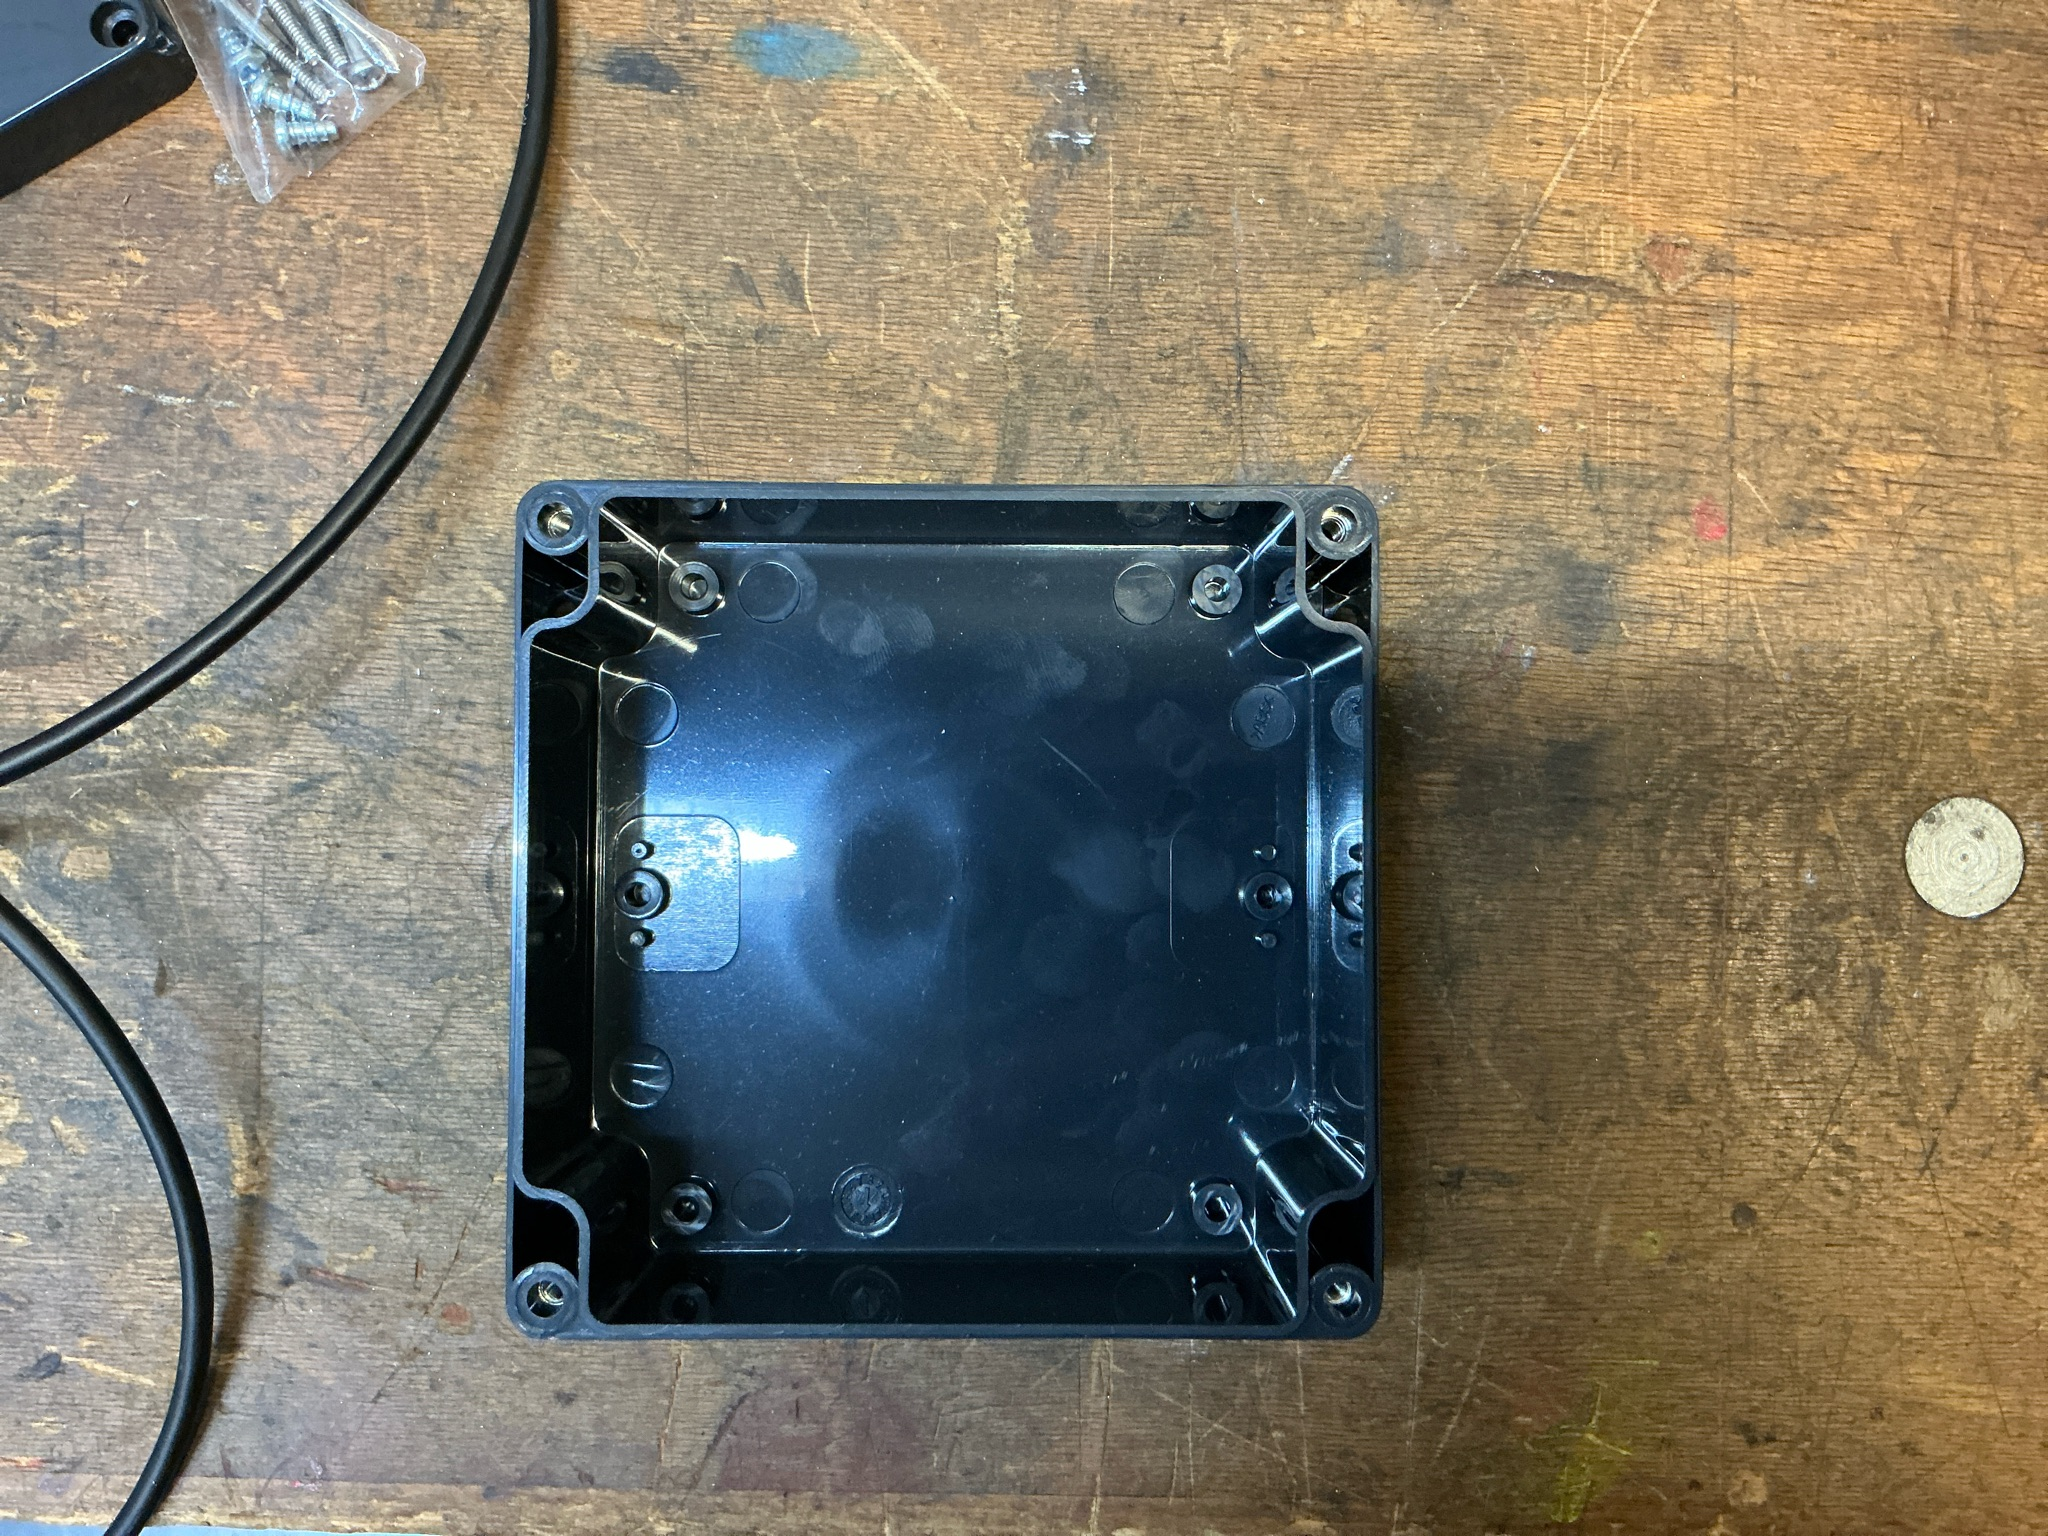
\includegraphics[width=0.45\textwidth, keepaspectratio]{box1.jpg}
        \caption[Urspr\"unglich vorgesehene Lenker-Box (Abbildungsverzeichnis)]{Urspr\"unglich vorgesehene Lenker-Box}
        %\footcite{VLInkManual}
        
        \label{fig:box1}
    \end{center}
\end{figure}

Da sich diese als für den gewünschten Einsatz zu groß dimensioniert herausstellt, sollte eine kleinere Box bestellt und verwendet werden, siehe Abbildung \ref{fig:dan1}.
Die kleinere Box hat die Aussenmasse 120 x 80 x 55 mm. Die zu entwerfende Platine (siehe Kapitel \ref{sec:fahrradplatine}) sollte so dimensioniert sein, dass sie in dieser kleineren Box Platz findet, daher musste auch diese neu entworfen werden.

\begin{figure}[h]
    \begin{center}
        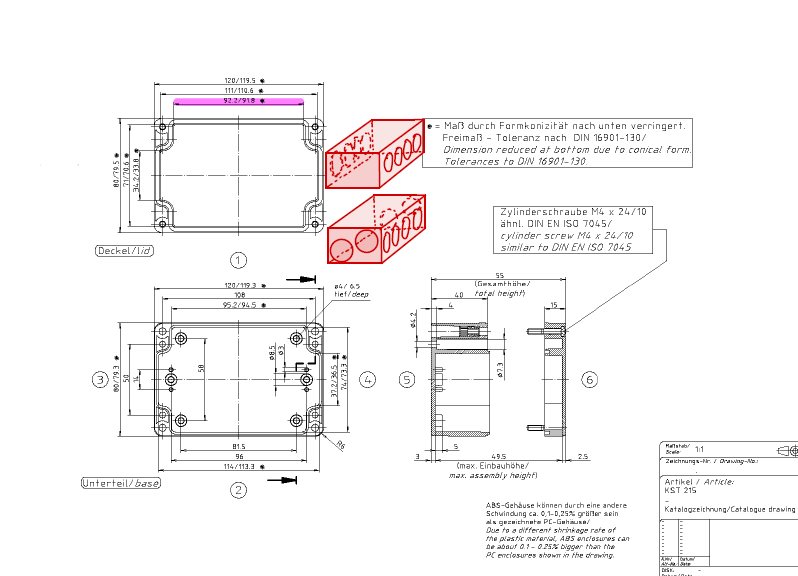
\includegraphics[width=0.7\textwidth, keepaspectratio]{dan1.png}
        \caption[Kleinere Lenker-Box (Abbildungsverzeichnis)]{Kleinere Lenker-Box}
        %\footcite{VLInkManual}
        
        \label{fig:dan1}
    \end{center}
\end{figure}

\newpage{}
\subsection{Platinendesign Fahrrad \(Bellgardt\)}
\label{sec:fahrradplatine}
Zu Beginn sind wir davon ausgegangen, dass die DMS direkt mit der neuen Messtechnik verbunden werden können, siehe Abbildung \ref{fig:fab5}.
\begin{figure}[h]
    \begin{center}
        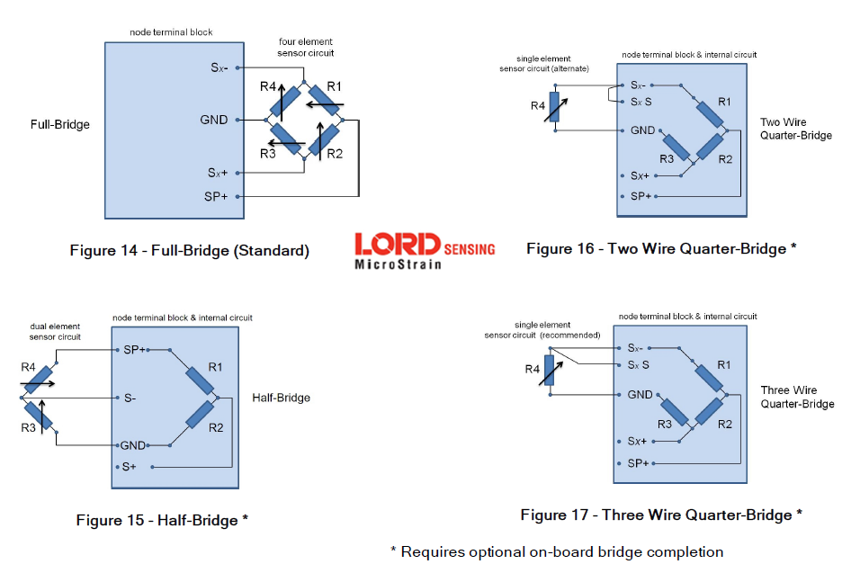
\includegraphics[width=0.9\textwidth, keepaspectratio]{fab5.png}
        \caption[LORD Konfigurationen der Brücken (Abbildungsverzeichnis)]{LORD Konfigurationen der Brücken}
        \footcite{VLInkManual
        }
        
        \label{fig:fab5}
    \end{center}
\end{figure}

Da dies nicht möglich ist, haben wir als Lösung eine Zwischenplatine konstruiert, welche die DMS mit zwei Widerständen zur Halbbrücke ergänzt, siehe Abbildung \ref{fig:fab6}.

\begin{figure}[h]
    \begin{center}
        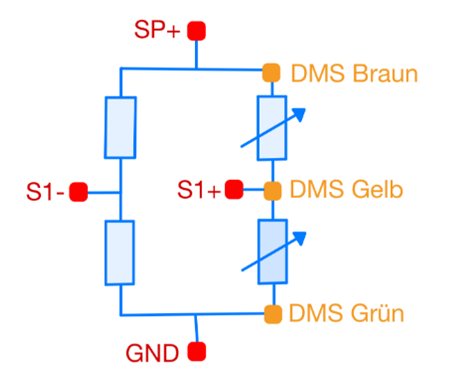
\includegraphics[width=0.4\textwidth, keepaspectratio]{fab6.png}
        \caption[Schaltplan Protoyp Platine (Abbildungsverzeichnis)]{Schaltplan Protoyp Platine}
        %\footcite{VLInkManual
        %}
        
        \label{fig:fab6}
    \end{center}
\end{figure}

Für die Messtechnik sieht dies nun aus wie eine Vollbrücke. Um uns das Wirkungsprinzip und die Funktionsfähigkeit zu verdeutlichen, wurde die Schaltung für den Biegebalken konstruiert.
Der Mittelabgriff des Biegebalkens ist dabei die gelbe Ader. Die Versorgungsapannung von 4,096 V wird durch die Messtechnik vorgegeben und liegt zwischen den Kontakten SP+ und GND an. Der Brückenausgang wird zwischen S1- und S1+ gemessen. Hierüber wird die Belastung der Brücke durch Dehnung der DMS in eine Spannung zwischen S1- und S1+ dargestellt
\subsubsection{Der erste Prototyp}
Basierend auf dem ersten Schaltungsplan wurde dann eine Prototyp-Platine erstellt. Die Platine basiert auf einer Lochplatine.
Die verwendeten Widerstände sind 120 Ohm-Metallschichtwiderstände mit einer Abweichung von 1 \%. Der Prototyp wurde am Biegebalken getestet.
\begin{figure}[h]
    \begin{center}
        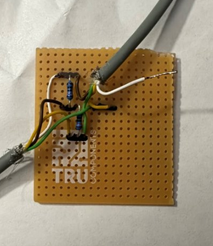
\includegraphics[width=0.4\textwidth, keepaspectratio]{fab7.png}
        \caption[Prototyp Platine mit der Ergänzung der DMS zur Halbbrücke (Abbildungsverzeichnis)]{Prototyp Platine mit der Ergänzung der DMS zur Halbbrücke}
        %\footcite{VLInkManual
        %}
        
        \label{fig:fab7}
    \end{center}
\end{figure}



\subsubsection{Platinenplanung der Lenkerbox}
Der alte Aufbau hat einige Eigenschaften, die durch den neuen Aufbau verbessert wurden. So wurde der alte Aufbau auf einer Lochplatine realisiert.
Zudem wurde die Verbindung der Platine mit Schraubklemmen gelöst.

\begin{figure}[h]
    \begin{center}
        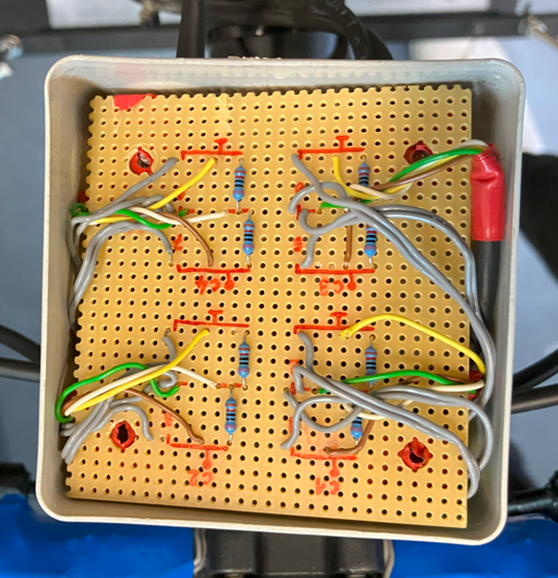
\includegraphics[width=0.3\textwidth, keepaspectratio]{fab8.png}
        \caption[Alte Platine in der alten Lenkerbox (Abbildungsverzeichnis)]{Alte Platine in der alten Lenkerbox}
        %\footcite{VLInkManual
        %}
        
       \label{fig:fab8}
    \end{center}
\end{figure}

Viele der angemerkten Punkte konnten verbessert werden. Hierzu wurde zunächst der Schaltplan in der Software KiCad\cite{KiCadWebsite} eingepflegt.

\begin{figure}[h]
    \begin{center}
        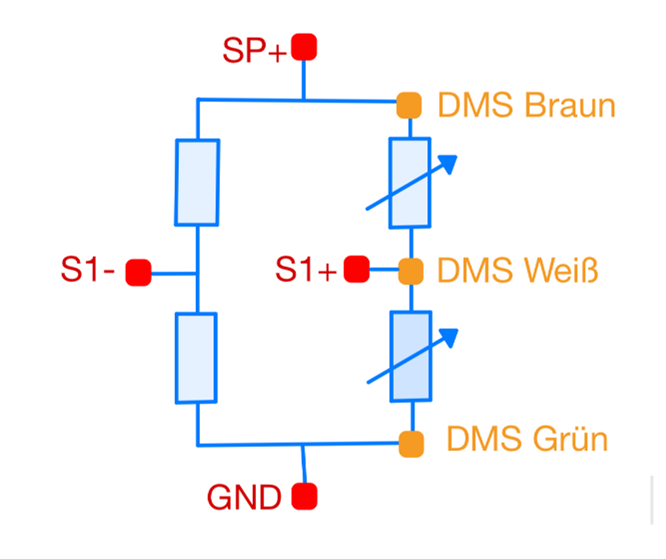
\includegraphics[width=0.3\textwidth, keepaspectratio]{fab9.png}
        \caption[Schaltungsplan Fahrrad (Abbildungsverzeichnis)]{Schaltungsplan Fahrrad}
        %\footcite{VLInkManual
        %}
        
        \label{fig:fab9}
    \end{center}
\end{figure}

\subsubsection{Planung der Schaltung mit KiCAD}
In der Software KiCad\cite{KiCadWebsite} wurde zunächst ein Schaltplan erstellt, siehe Abbildung \ref{fig:fab11}.
KiCad ist ein freies Tool, mit dem man Platinen planen kann. Nach dem erfolgreichen Test der Prototyp Platine am Biegbalken wurde die Schaltung hochskaliert. Der Hauptunterschied im Anschluss der DMS des Biegebalkens und denen des Fahrrads besteht darin, dass der Mittelabgriff am Fahrrad durch die weißen DMS bereitgestellt wird.

\begin{figure}[htbp]
    \begin{center}
        
\includegraphics[width=0.2\textwidth, keepaspectratio]{fab10.png}
        \caption[KiCad Software Logo (Abbildungsverzeichnis)]{KiCad Software Logo}
        \cite{KiCadWebsite}
        \label{fig:fab10}
    \end{center}
\end{figure}


Dieser stellt vier Halbbrücken dar.
Auf der Platine werden pro Halbbrücke je zwei Widerstände angebracht. Diese befinden sich in Form ihrer Kontakte auf der Platine.
Basierend auf dem Schaltplan (siehe Anhang \ref{sec:schaltplan2}) wurde dann die Platine zunächst entsprechend Ihrer Abmessungen für das Gehäuse simuliert (siehe Abbildung \ref{fig:fab12}) und anschließend gedruckt. Die fertige Platine ist in der Abbildung \ref{fig:fab13} zu sehen. Sie besitzt die Maße des Gehäuses. Zudem verfügt die Platine über vier zusätzliche Bohrungen, um sie besser im Gehäuse befestigen zu können. 
\begin{figure}[htbp]
    \centering
    \begin{minipage}{0.48\textwidth}
        \centering
        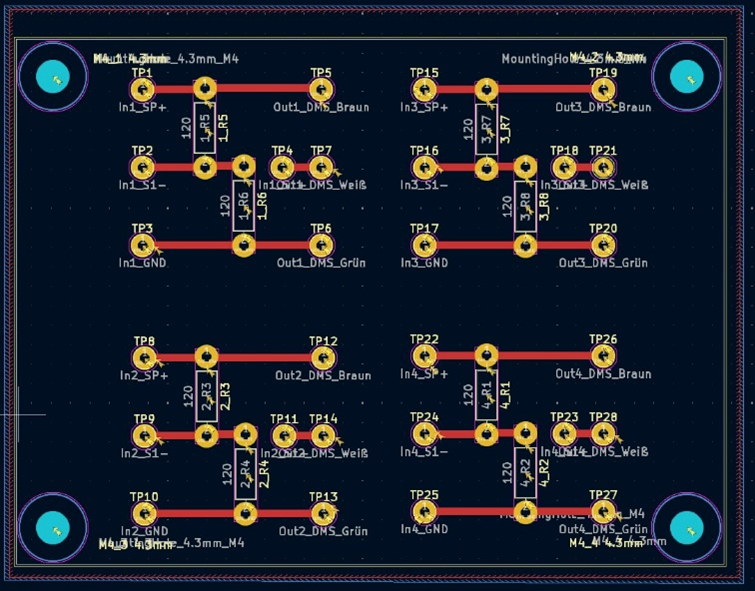
\includegraphics[width=\textwidth, keepaspectratio]{fab11.png}
        \caption[Planung Lenkerplatine (Abbildungsverzeichnis)]{Planung Lenkerplatine}
        \label{fig:fab11}
    \end{minipage}
    \hfill
    \begin{minipage}{0.48\textwidth}
        \centering
        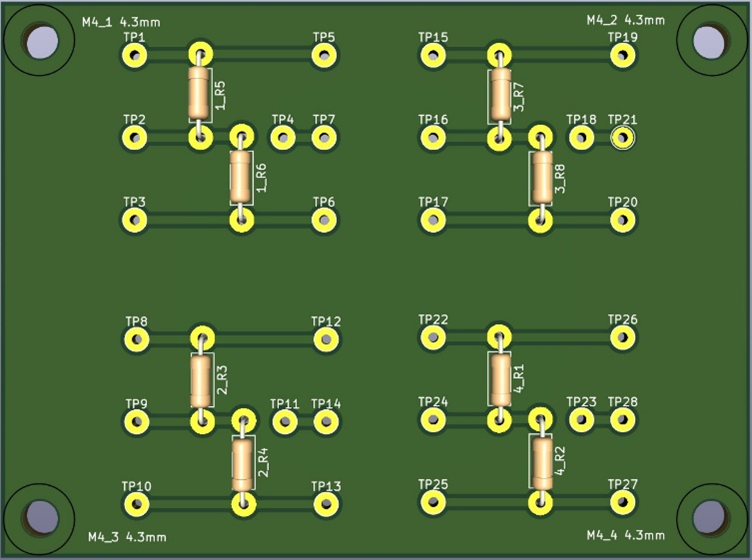
\includegraphics[width=\textwidth, keepaspectratio]{fab12.png}
        \caption[Simulation der Lenkerplatine (Abbildungsverzeichnis)]{Simulation der Lenkerplatine}
        \label{fig:fab12}
    \end{minipage}
    %\caption{Gegenüberstellung: Planung (links) und Simulation (rechts) der Lenkerplatine.}
\end{figure}


\begin{figure}[htbp]
    \begin{center}
        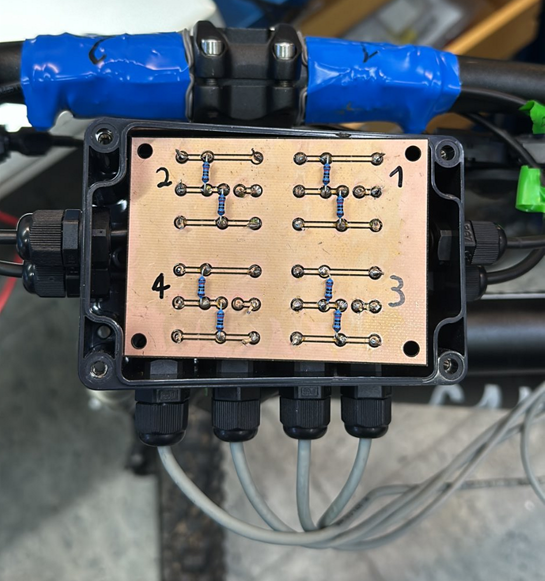
\includegraphics[width=0.5\textwidth, keepaspectratio]{fab13.png}
        \caption[Fertig installierte Lenkerplatine (Abbildungsverzeichnis)]{Fertig installierte Lenkerplatine}
        %\footcite{www.kicad.org}
        \label{fig:fab13}
    \end{center}
\end{figure}


\newpage
\subsection{Platinendesign Suit \(Nerb, Ulit\)}
Die Schaltung für den Flying Suit wurde basierend auf der zuvor geplanten Vollbrückenschaltung entwickelt.
Es wurden zwei SMD-Metallschichtwiderstände verwendet, da diese eine kompakte Bauform haben und eine hohe Langzeitstabilität gewährleisten.
Die gesamte Schaltung wurde mit Cadence OrCAD Capture für den Schaltplan erstellt und anschließend in Allegro PCB Designer für das Platinenlayout umgesetzt.
Zunächst wurde die Schaltung in OrCAD Capture entworfen und die Platinengröße basierend auf dem verfügbaren Platz im Platinengehäuse festgelegt.
Dabei wurden zwei Bohrungen berücksichtigt, um die Platine mit Schrauben sicher im Gehäuse zu befestigen.
Zudem wurden Leiterplattenklemmen integriert, um die Leitungen einfach anschließen zu können.
Diese Lösung erleichtert spätere Modifikationen oder den Austausch von Komponenten, da keine Verbindungen ausgelötet werden müssen.
Die folgende Schaltplan-Darstellung zeigt den elektrischen Aufbau der Platine für den Flying Suit.
Die Dehnungsmessstreifen (DMS) sind entsprechend der Vollbrückenschaltung integriert, während die Metallschichtwiderstände zur Signalverarbeitung beitragen.
Die Anschlüsse sind klar gekennzeichnet, um eine einfache Verdrahtung zu ermöglichen.
\subsubsection{Fertigungsprozess der Platine}
\begin{enumerate}
    \item Erstellung des Schaltplans in Cadence OrCAD Capture.
    \item Definition der Platinengröße basierend auf dem Gehäusemaß.
    \item Platzierung der SMD-Widerstände und anderer Komponenten in Allegro PCB Designer.
    \item Integration von Bohrungen für die Befestigungsschrauben.
    \item Ergänzung von Leiterplattenklemmen zur vereinfachten Verdrahtung.
    \item Herstellung der Platine und Bestückung mit den Komponenten.
    \item Validierung der Schaltung durch Funktionsprüfung.
\end{enumerate}
Die gefertigte Platine wurde anschließend in das Gehäuse integriert und mit den notwendigen Bauteilen verbunden. Zur Validierung der Funktionalität wurde die Schaltung getestet und überprüft, um sicherzustellen, dass sie wie geplant funktioniert.
Die folgenden Abbildungen \ref{fig:un5}, \ref{fig:un5} und \ref{fig:un5} zeigen die gefertigte Platine, den Schaltplan sowie die finale Integration der Platine im Platinengehäuse.
\begin{figure}[htbp]
    \begin{center}
        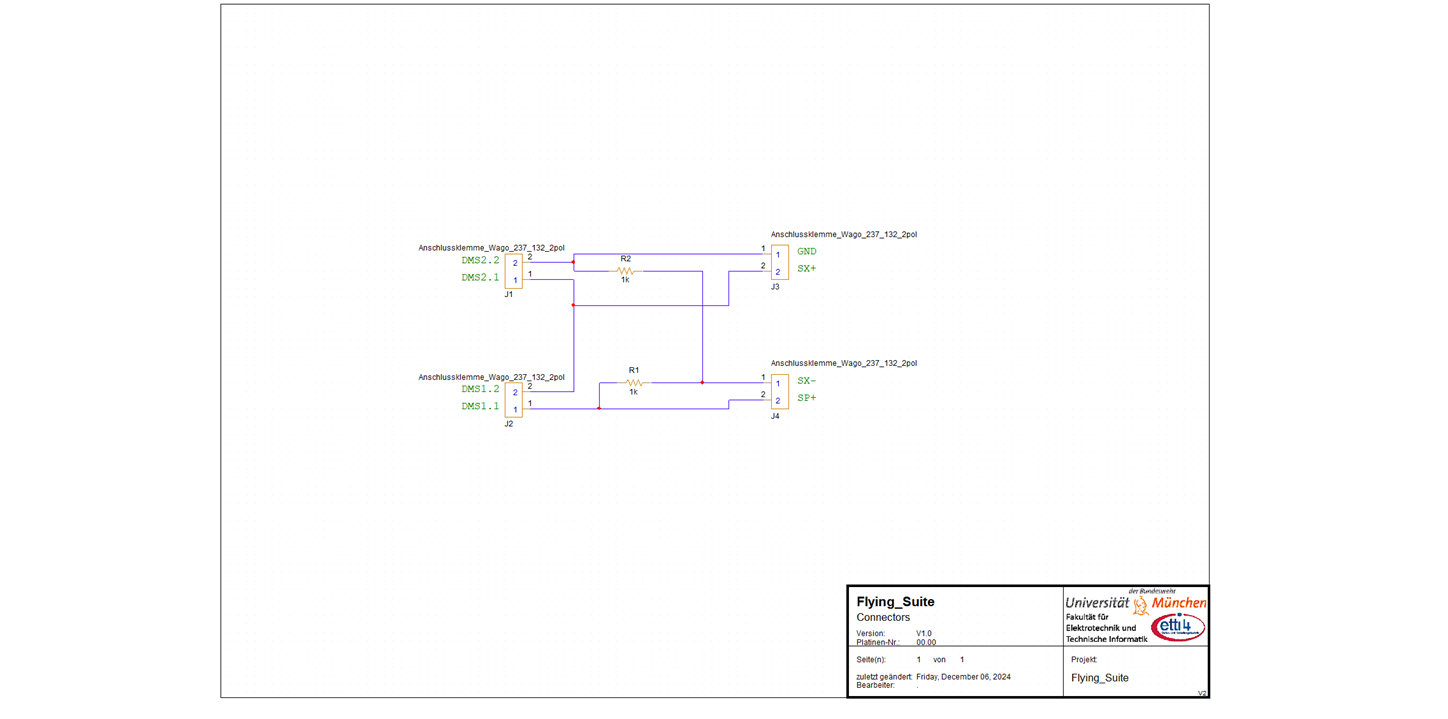
\includegraphics[width=1\textwidth, keepaspectratio]{un5.png}
        \caption[Schaltplan der Flying Suit Platine (Abbildungsverzeichnis)]{Schaltplan der Flying Suit Platine}
        %\footcite{www.kicad.org}
        \label{fig:un5}
    \end{center}
\end{figure}

\begin{figure}[htbp]
    \centering
    \begin{minipage}{0.48\textwidth}
        \centering
        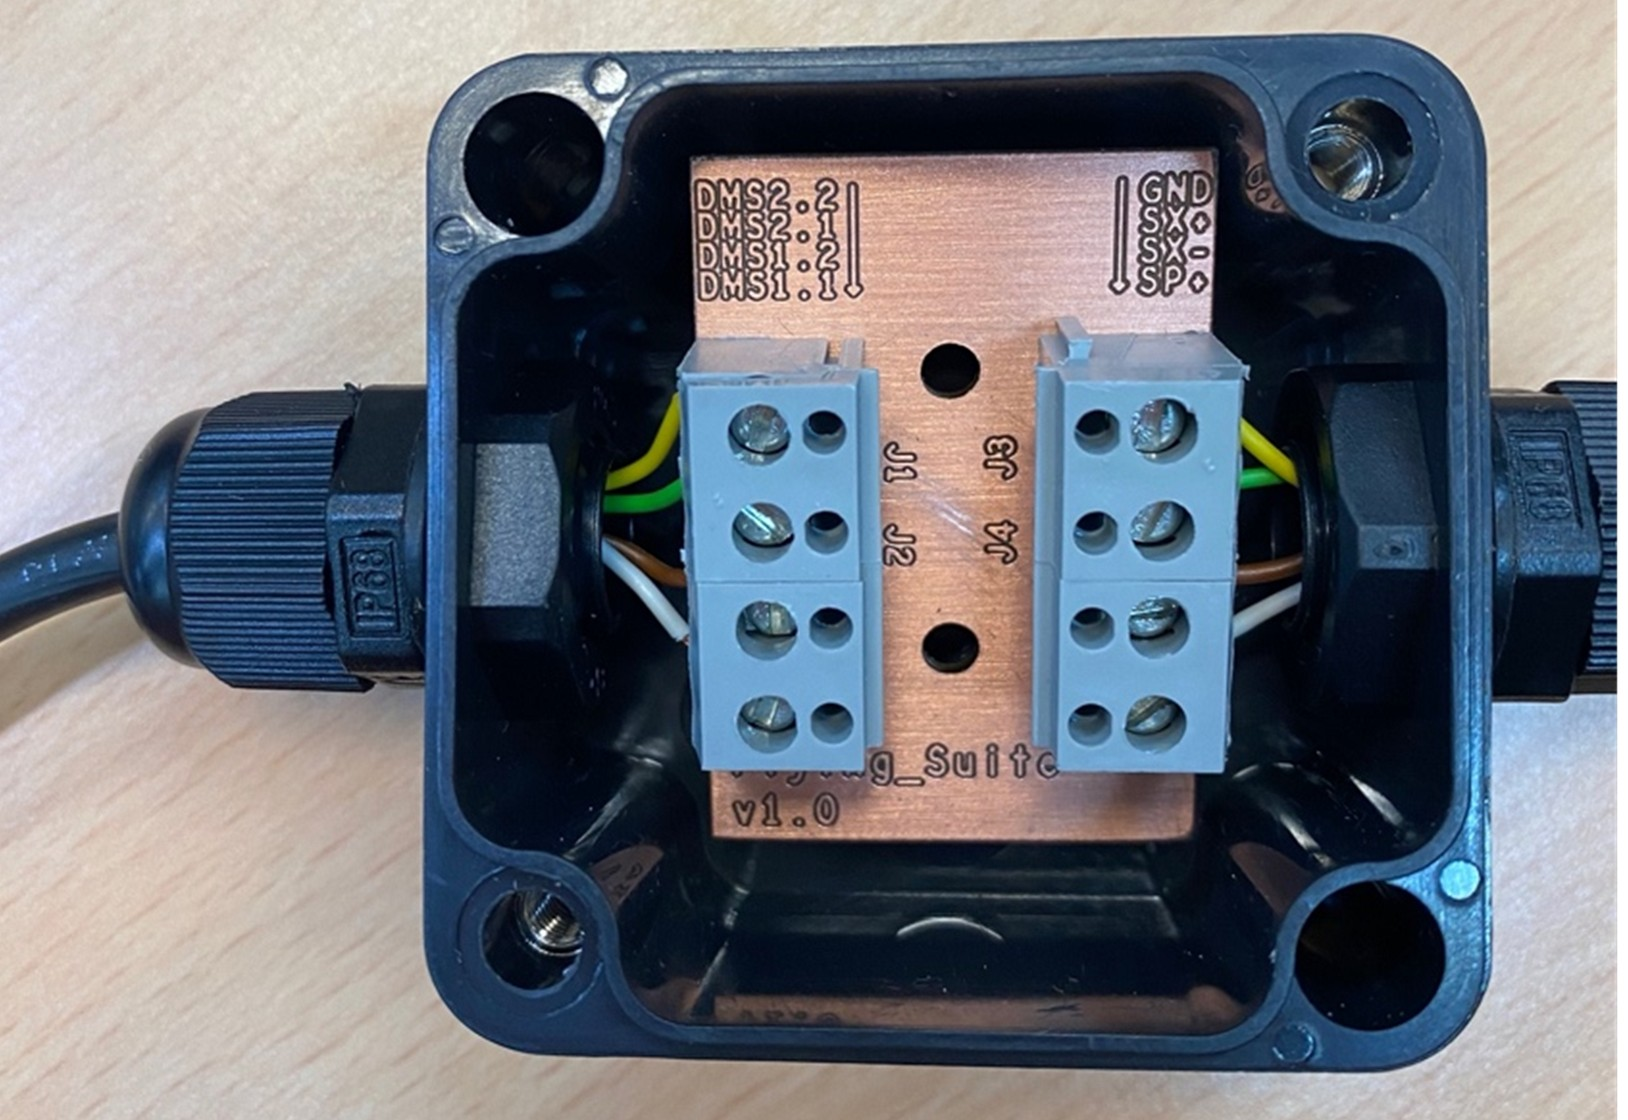
\includegraphics[width=\textwidth, keepaspectratio]{un6.jpg}
        \caption[Fertige Flying Suit Platine mit aufgelöteten SMD-Widerständen (Abbildungsverzeichnis)]{Fertige Flying Suit Platine mit aufgelöteten SMD-Widerständen}
        \label{fig:un6}
    \end{minipage}
    \hfill
    \begin{minipage}{0.48\textwidth}
        \centering
        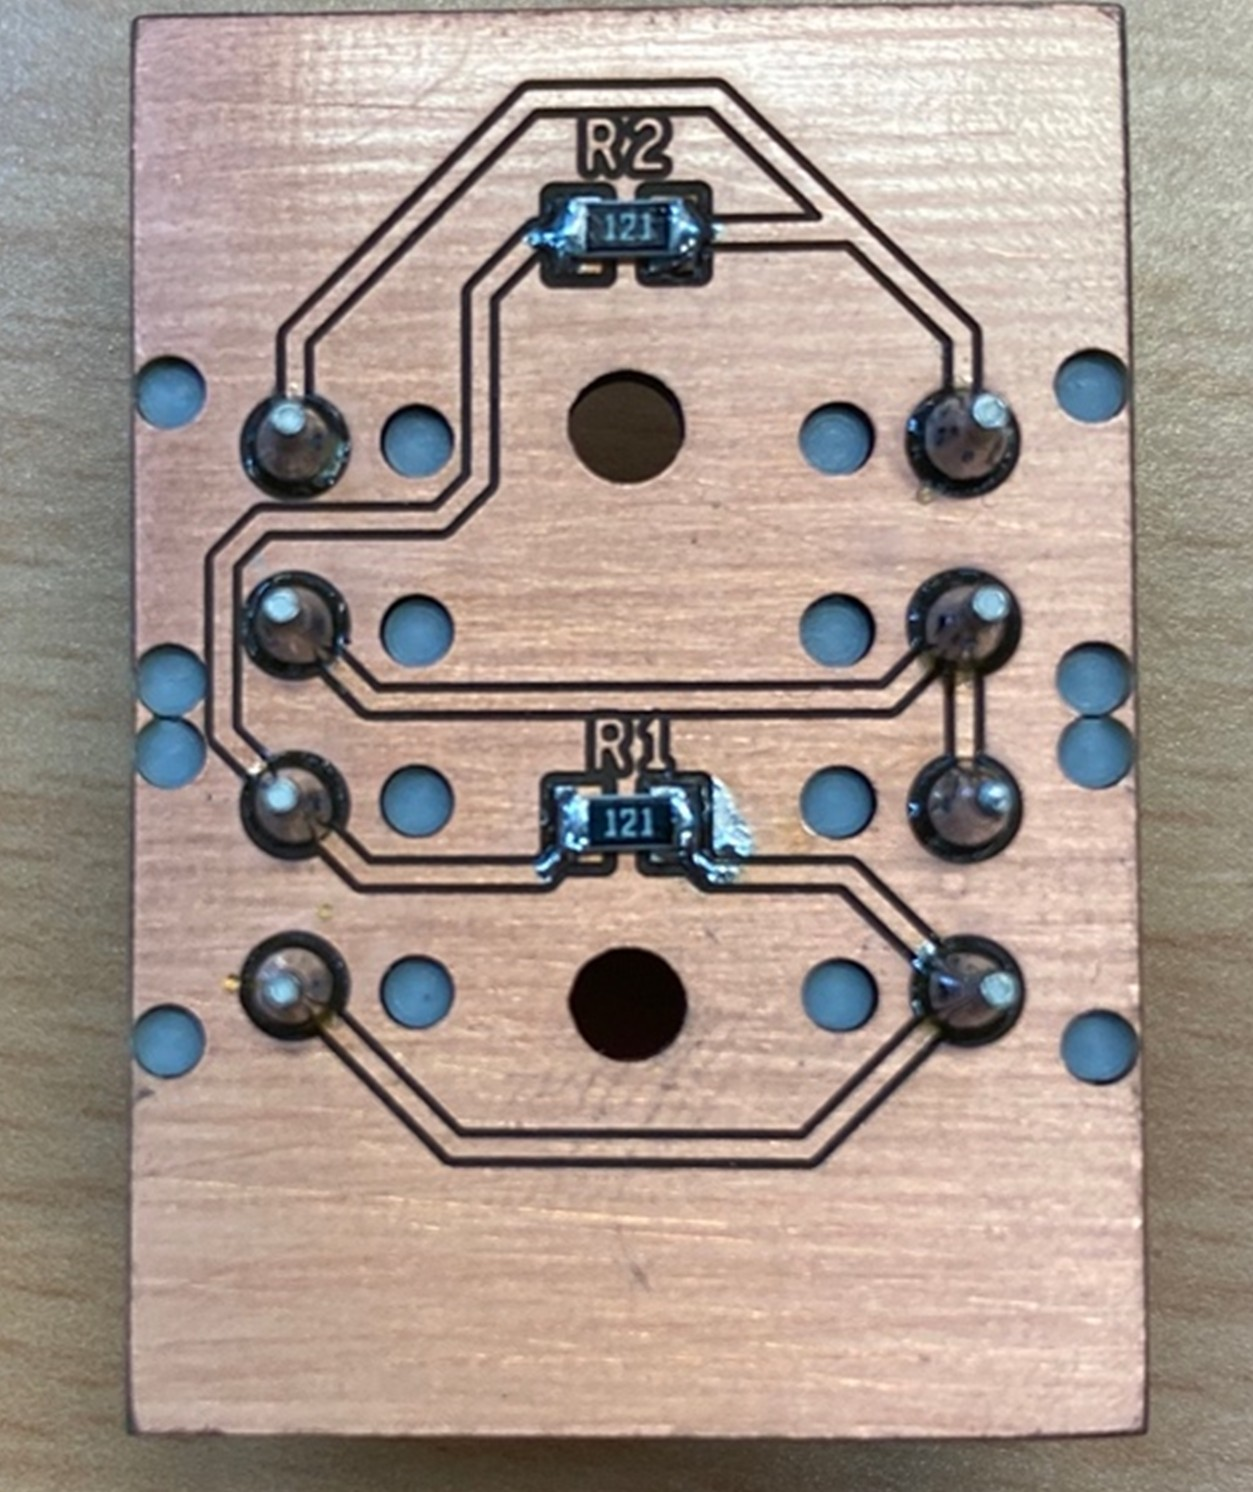
\includegraphics[width=\textwidth, keepaspectratio]{un7.jpg}
        \caption[Platine im Gehäuse mit verschraubten Leiterplattenklemmen (Abbildungsverzeichnis)]{Platine im Gehäuse mit verschraubten Leiterplattenklemmen}
        \label{fig:un7}
    \end{minipage}
\end{figure}



\newpage{}
\section{Herstellung der Acrylplatte f\"ur die Geh\"auseintegration \(Nerb, Ulit\)}
Um den V-Link 200 sicher im Gehäuse zu montieren, haben wir eine Acrylplatte als Befestigungsbasis konstruiert.
Dafür wurde zunächst das Gehäuse exakt vermessen und eine CAD-Zeichnung mit \textbf{CATIA V5} erstellt, siehe Abbildungen \ref{fig:un3} und \ref{fig:un4}.
\begin{figure}[htbp]
    \begin{center}
        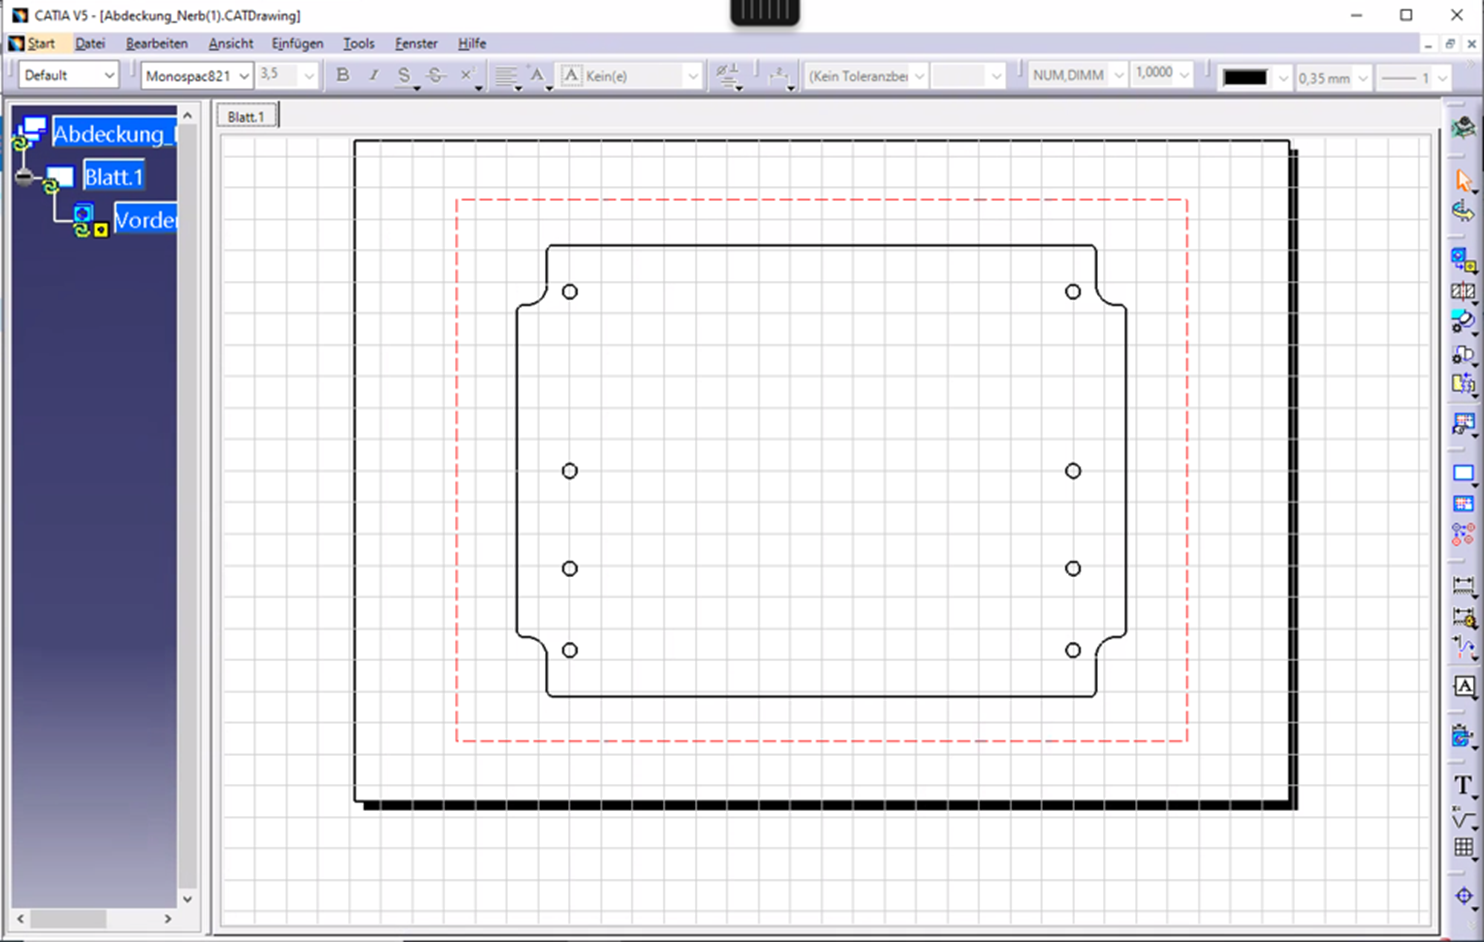
\includegraphics[width=0.75\textwidth, keepaspectratio]{un3.png}
        \caption[Acrylplatte Catia Draufsicht (Abbildungsverzeichnis)]{Acrylplatte Catia Draufsicht}
        %\footcite{www.kicad.org}
        \label{fig:un3}
    \end{center}
\end{figure}
\begin{figure}[htbp]
    \begin{center}
        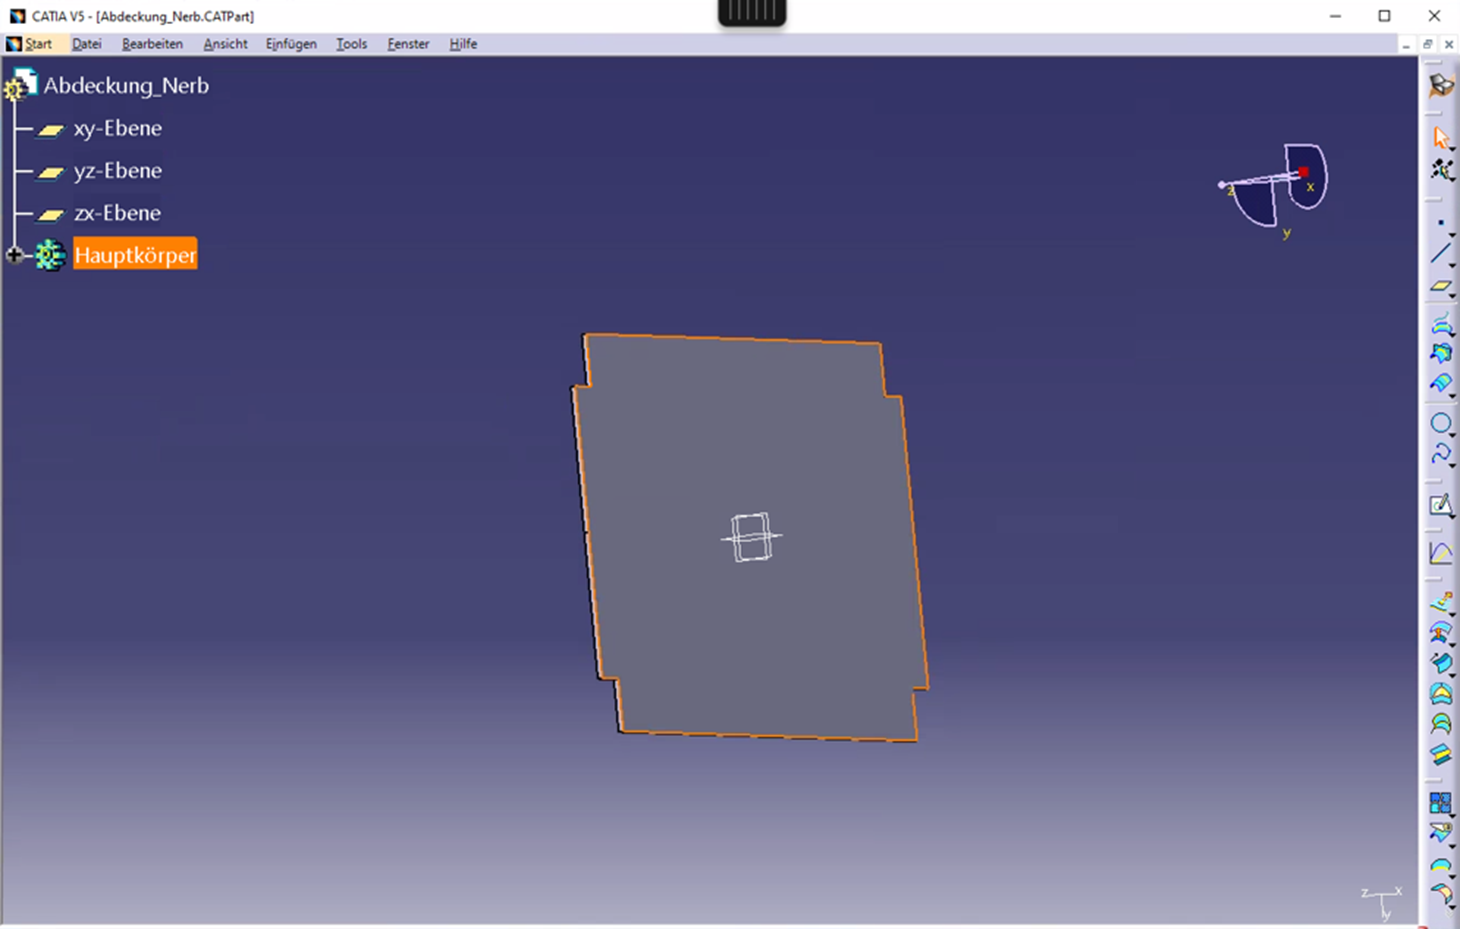
\includegraphics[width=0.75\textwidth, keepaspectratio]{un4.png}
        \caption[Acrylplatte Catia 3D Ansicht (Abbildungsverzeichnis)]{Acrylplatte Catia 3D Ansicht}
        %\footcite{www.kicad.org}
        \label{fig:un4}
    \end{center}
\end{figure}

Basierend auf dieser Zeichnung wurde die Acrylplatte mit einem Laser exakt zugeschnitten.
Es handelt sich um eine 3 mm dicke Acrylplatte, die an der Universität mittels Laserschneidtechnik aus den CAD-Daten gefertigt wurde.
Beim ersten Versuch wurden die exakten Innenmaße des Gehäuses verwendet, jedoch stellte sich heraus, dass die Platte nur schwergängig in das Gehäuse passte.
Daher wurde das Außenmaß der Acrylplatte um 0,5 mm reduziert, um eine bessere Passform zu gewährleisten.
Die Acrylplatte enthält mehrere Bohrungen, um den V-Link 200 sicher befestigen zu können.
Zwei Bohrungen wurden für die Montage des V-Link vorgesehen, an denen er mit M4-Feingewindeschrauben und Muttern fixiert wird.
Zusätzlich wurde ein Ausschnitt für den Einschaltknopf eingefügt, um eine einfache Bedienung zu ermöglichen.
Die Befestigung der Acrylplatte selbst im Gehäuse erfolgte mittels Flachkopfschrauben.
Diese Konstruktion gewährleistet eine stabile Fixierung des V-Link 200 und schützt ihn vor mechanischen Belastungen während des Messbetriebs.
Zudem ermöglicht die durchdachte Gestaltung der Acrylplatte eine einfache Entnahme und Wartung des Geräts, falls erforderlich.

\subsection{Fertigungsprozess der Acrylplatte}
\begin{enumerate}
    \item Vermessung des Gehäuses und Anfertigung der CAD-Zeichnung in CATIA V5.
    \item Laserschneiden der Acrylplatte gemäß den CAD-Daten an der Universität.
    \item Bohren der Montagelöcher für den V-Link 200.
    \item Einfügen eines Ausschnitts für den Einschaltknopf.
    \item Fixierung des V-Link 200 mit Feingewindeschrauben und Muttern.
    \item Montage der Acrylplatte im Gehäuse mit Flachkopfschrauben.
\end{enumerate}


\newpage
\section{Montage und Verbindung der DMS \(Nerb, Ulit\)}
Die Montage der Dehnungsmessstreifen (DMS) erfolgte in mehreren Schritten, um eine präzise und zuverlässige Messung zu gewährleisten.
Zunächst wurden die Oberflächen der Messstellen sorgfältig mit Schleifpapier gesäubert und anschließend mit Alkohol gereinigt, um eine optimale Haftung der DMS zu ermöglichen.

Bei den Dehnungsmessstreifen für \textbf{Biegung} wurden jeweils zwei DMS an gegenüberliegenden Seiten der Struktur aufgebracht, um eine symmetrische Messung zu gewährleisten.
Im Gegensatz dazu wurde der \textbf{DMS für die Torsion} nur an einer Stelle angebracht.
Nach der Reinigung wurde der Kleber aufgetragen, und die DMS wurden mithilfe von Tesa exakt positioniert und fixiert.
Nach der Aushärtung des Klebers wurden Lötstützpunkte aufgebracht, um eine stabile Verbindung mit der Steuerleitung herzustellen.
Anschließend wurden die Widerstände der DMS gemessen, um sicherzustellen, dass die Werte innerhalb der erwarteten Toleranzen liegen.
Die Verbindung zur Platine erfolgte über die Lötstützpunkte und wurde anschließend an die integrierten Leiterplattenklemmen angeschlossen,
wodurch eine flexible und austauschbare Lösung geschaffen wurde.
Nach der Montage wurden alle Verbindungen überprüft, um sicherzustellen, dass die Signale korrekt erfasst und weitergeleitet werden.

\subsection{Fertigungsprozess der DMS-Verbindung}
\begin{enumerate}
    \item Reinigung der Oberfläche mit Schleifpapier (Körnung 180) und Alkohol.
    \item Aufbringen der Dehnungsmessstreifen (DMS) mit speziellem Kleber und Fixierung mit Tesa.
    \item Aushärtung des Klebers und erste Sichtprüfung.
    \item Unmittelbare Messung der DMS nach dem Aufbringen.
    \item Anbringung von Lötstützpunkten zur sicheren Verbindung mit der Steuerleitung.
    \item Verbindung zur Platine über Leiterplattenklemmen.
    \item Widerstandsmessung zur Überprüfung der elektrischen Eigenschaften.
    \item Endprüfung aller Verbindungen zur Sicherstellung der Messgenauigkeit.
\end{enumerate}
Abbildungen \ref{fig:un8} und \ref{fig:un9} zeigen die angebrachten DMS.

\begin{figure}[htbp]
    \centering
    \begin{minipage}{0.48\textwidth}
        \centering
        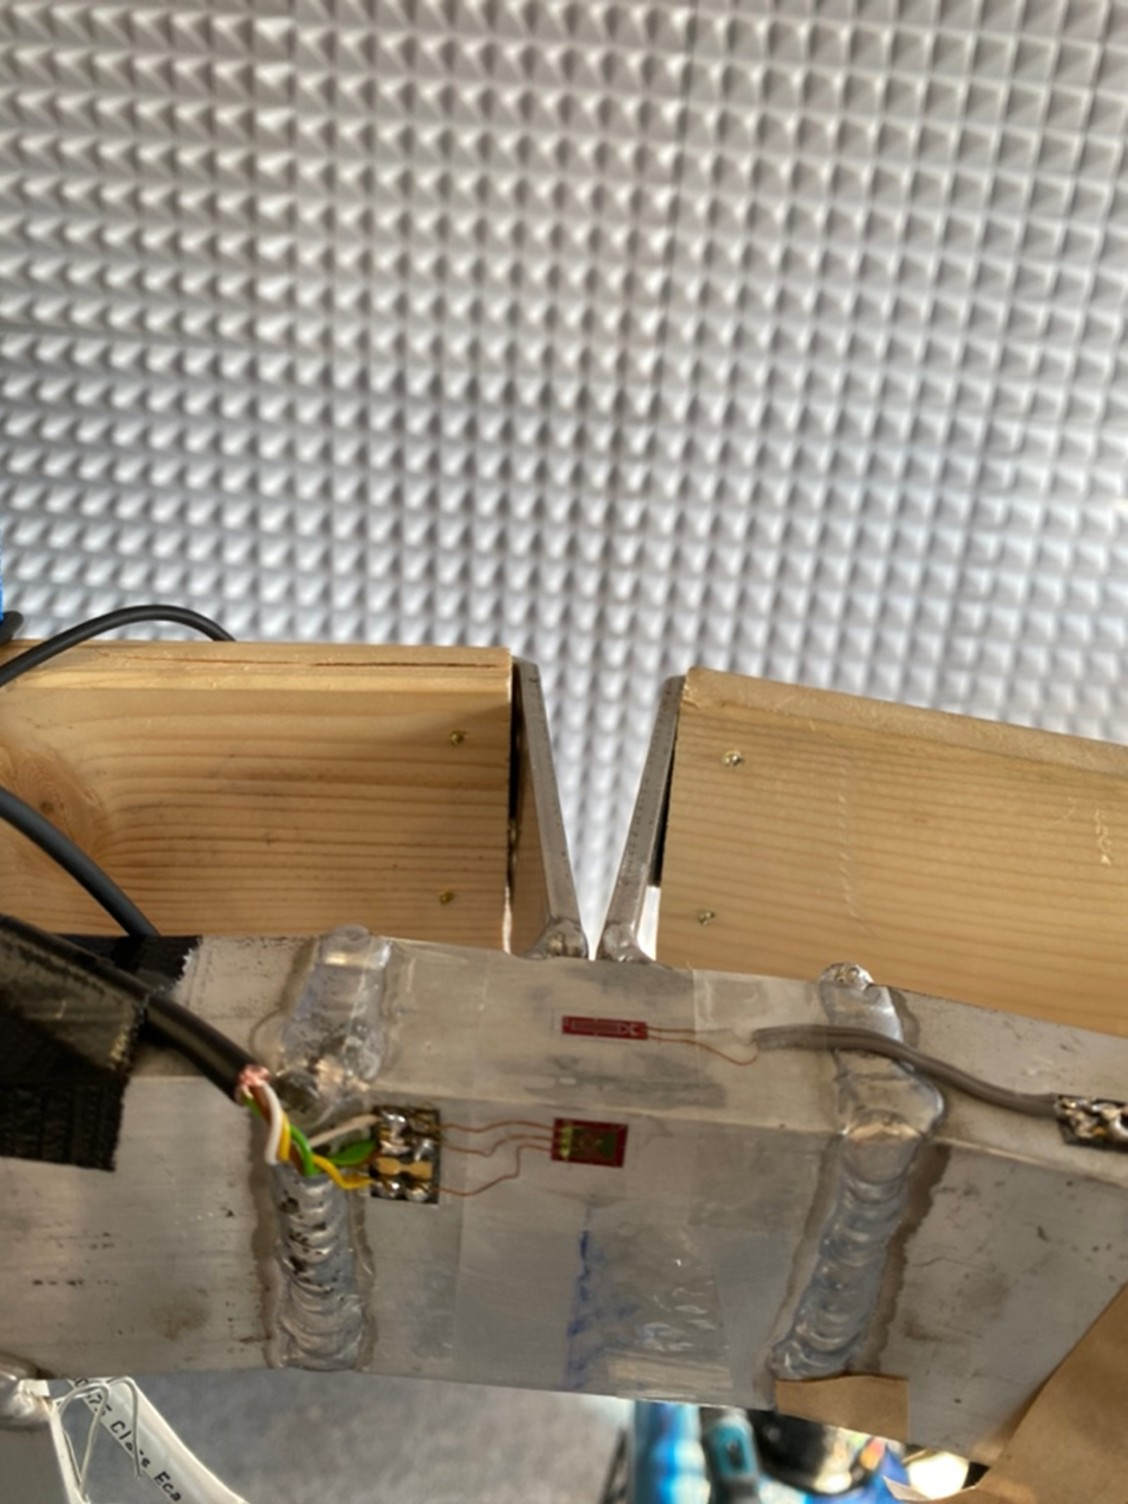
\includegraphics[width=\textwidth]{un8.jpg}
        \caption[Am Flying Suit angebrachte DMS 1]{Am Flying Suit angebrachte DMS 1}
        \label{fig:un8}
    \end{minipage}
    \hfill
    \begin{minipage}{0.48\textwidth}
        \centering
        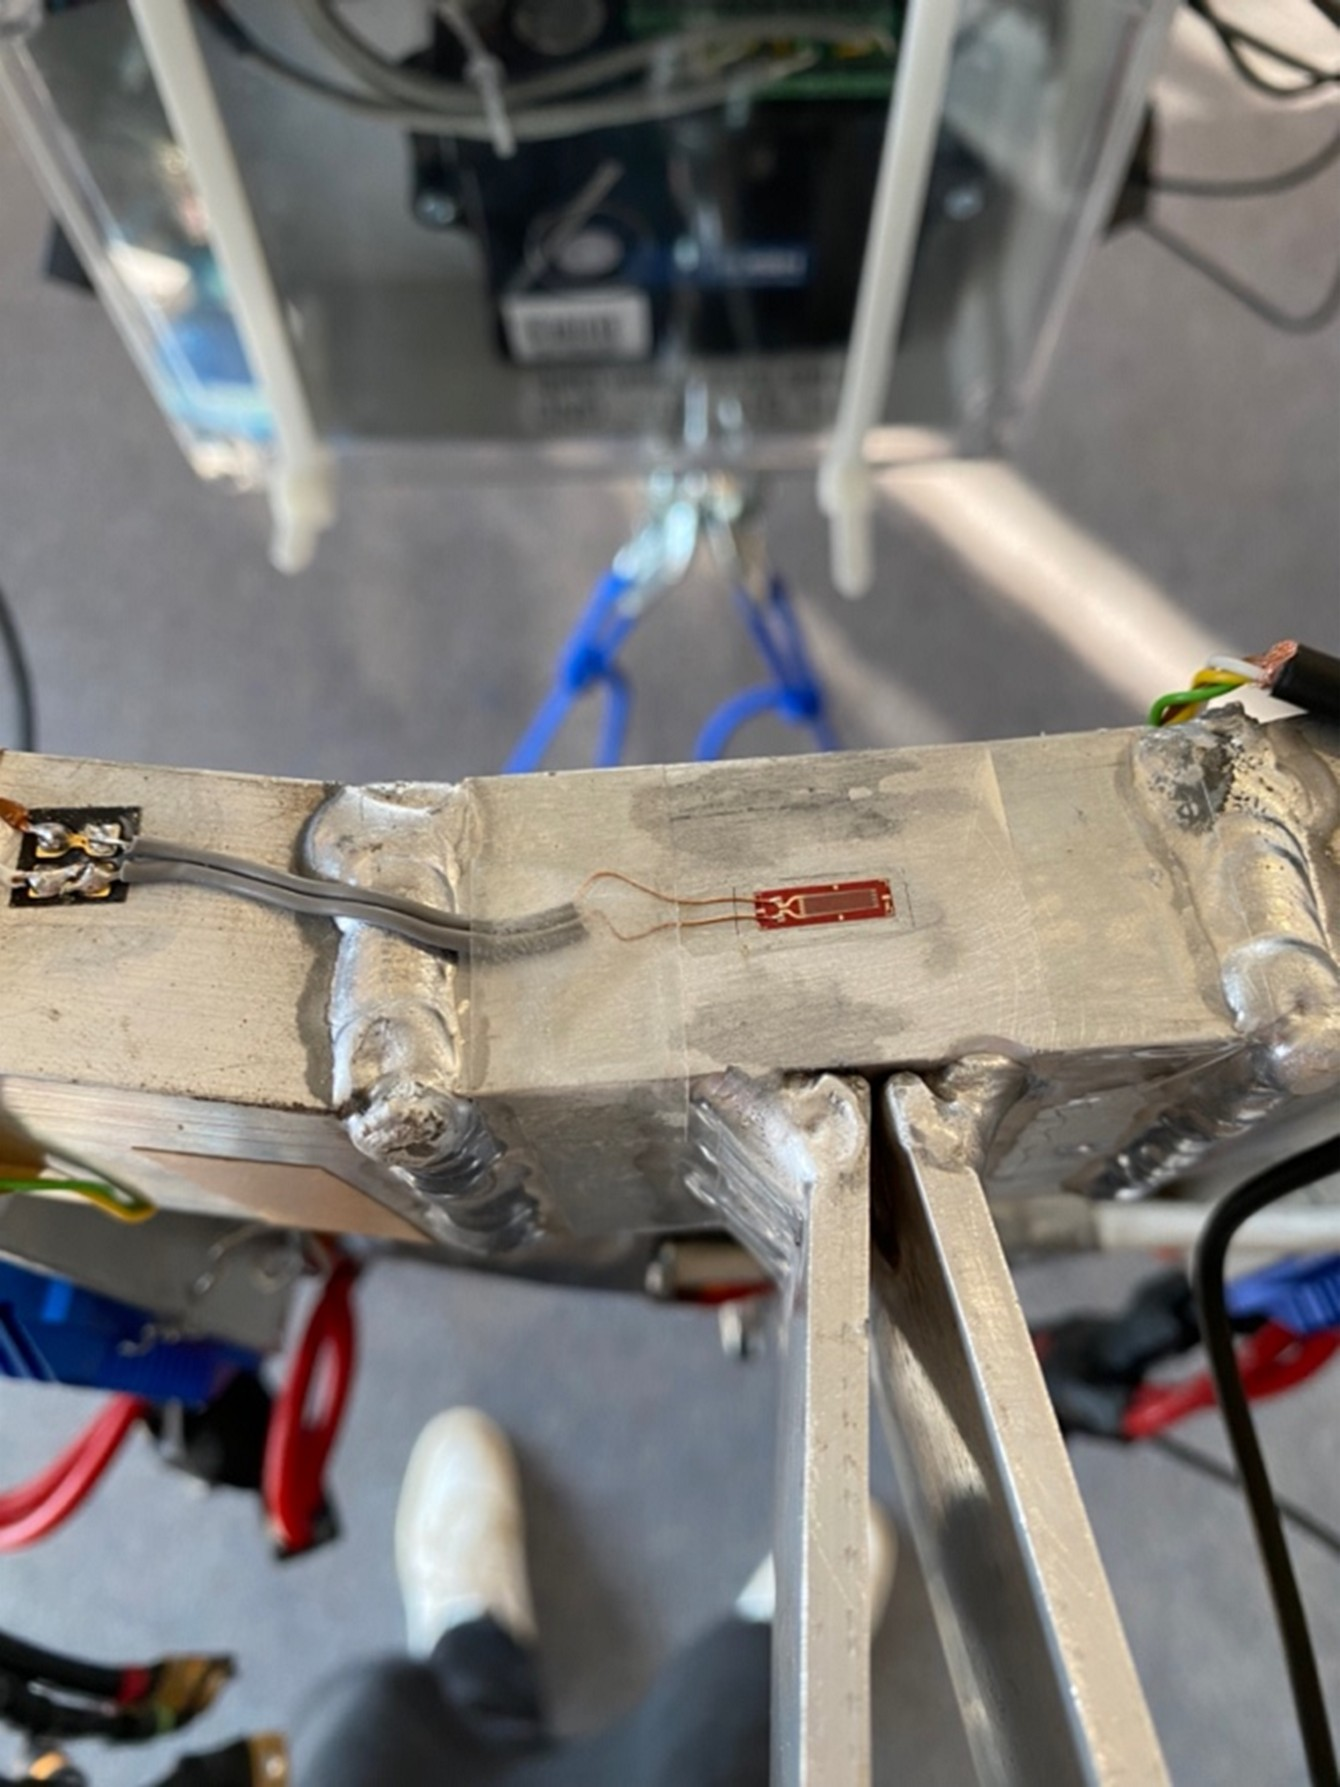
\includegraphics[width=\textwidth]{un9.jpg}
        \caption[Am Flying Suit angebrachte DMS 2]{Am Flying Suit angebrachte DMS 2}
        \label{fig:un9}
    \end{minipage}
\end{figure}

